%%%%%%%%%%%%%%%%%%%%%%%%%%%%%%%%%%%%%%%%%%%%%%%%%%%%%%%%%%%%%%%%%%%%%%%%%%%%
% AGUtmpl.tex: this template file is for articles formatted with LaTeX2e,
% Modified November 2013
%
% This template includes commands and instructions
% given in the order necessary to produce a final output that will
% satisfy AGU requirements.
%
% PLEASE DO NOT USE YOUR OWN MACROS
% DO NOT USE \newcommand, \renewcommand, or \def.
%
% FOR FIGURES, DO NOT USE \psfrag
%
%%%%%%%%%%%%%%%%%%%%%%%%%%%%%%%%%%%%%%%%%%%%%%%%%%%%%%%%%%%%%%%%%%%%%%%%%%%%
%
% All questions should be e-mailed to latex@agu.org.
%
%%%%%%%%%%%%%%%%%%%%%%%%%%%%%%%%%%%%%%%%%%%%%%%%%%%%%%%%%%%%%%%%%%%%%%%%%%%%
%
% Step 1: Set the \documentclass
%
% There are two options for article format: two column (default)
% and draft.
%
% PLEASE USE THE DRAFT OPTION TO SUBMIT YOUR PAPERS.
% The draft option produces double spaced output.
%
% Choose the journal abbreviation for the journal you are
% submitting to:

% jgrga JOURNAL OF GEOPHYSICAL RESEARCH
% gbc   GLOBAL BIOCHEMICAL CYCLES
% grl   GEOPHYSICAL RESEARCH LETTERS
% pal   PALEOCEANOGRAPHY
% ras   RADIO SCIENCE
% rog   REVIEWS OF GEOPHYSICS
% tec   TECTONICS
% wrr   WATER RESOURCES RESEARCH
% gc    GEOCHEMISTRY, GEOPHYSICS, GEOSYSTEMS
% sw    SPACE WEATHER
% ms    JAMES
% ef    EARTH'S FUTURE
%
%
%
% (If you are submitting to a journal other than jgrga,
% substitute the initials of the journal for "jgrga" below.)

\documentclass[grl]{agutexSI}

\usepackage{rotating}


% Author names in capital letters:
\authorrunninghead{HUANG ET AL.}

% Shorter version of title entered in capital letters:
\titlerunninghead{IRRIGATION IMPACTS IN VR-CESM}

%Corresponding author mailing address and e-mail address:
%\authoraddr{Corresponding author: A. B. Smith,
%Department of Hydrology and Water Resources, University of
%Arizona, Harshbarger Building 11, Tucson, AZ 85721, USA.
%(a.b.smith@hwr.arizona.edu)}

\begin{document}

%% ------------------------------------------------------------------------ %%
%
%  TITLE
%
%% ------------------------------------------------------------------------ %%

%\includegraphics{agu_pubart-white_reduced.eps}

%%%%%%%%%%%%%%%%%%%%%%%%%%%%%%%%

%%% To be entered by author:

%% May use \\ to break lines in title:
% Author names in capital letters:
\title{Supporting Information for ``Anthropogenic Warming Impacts on Today's Sierra Nevada Snowpack and Flood Risk''}

%% ------------------------------------------------------------------------ %%
%
%  BEGIN ARTICLE
%
%% ------------------------------------------------------------------------ %%

% The body of the article must start with a \begin{article} command
%
% \end{article} must follow the references section, before the figures
%  and tables.

\begin{article}

%% ------------------------------------------------------------------------ %%
%
%  TEXT
%
%% ------------------------------------------------------------------------ %%



\noindent\textbf{Contents of this file}
%%%Remove or add items as needed%%%
\begin{enumerate}
\item Figure S1
\item Figure S2
\item Figure S3
\item Figure S4
%if Tables are larger than 1 page, upload as separate excel file
\end{enumerate}
\ \\

\noindent\textbf{Introduction}


This supporting information includes:

\begin{itemize}

\item[1)]  Figure S1: Figure depicting the warming patterns averaged from Oct. to March. based on the CMIP5 ensemble mean compared to the recent historical for the natural, RCP4.5, and RCP8.5.

%the averaged precipitation and April 1st SWE from WRF at 27 km, and 

\item[2)]  Figure S2: Figure depicting the station locations for the observed precipitation and April 1st SWE (note: for the SWE, the black dots refer to the stations with data of the season 2015-2016 and green stars refer to the ones of the season 2016-2017).

\item[3)]  Figure S3: Figure depicting the model evaluation of the simulated Pr and SWE according to the station observations and the corresponding simulated values over the Sierra Nevada, and the relevant spatial pattern of the model output. For the drier year of 2015-2016, the relative bias between the model and observations averaged over all the stations is around 21$\%$, with a mean observed Pr of 5.7 mm$/$day. For the extremely wet year of 2016-2017, the average bias is around 2.4 mm/day, compared to the mean observed Pr of 11.6 mm$/$day. For April 1st SWE, the model underestimates SWE somewhat in 2016 with an average underestimation of 155.7 mm, compared to the mean observed SWE of 645.8 mm. For year 2017, the average bias is around 231.7 mm compared to the mean observed SWE of 1248.4 mm, or about 24$\%$.

\item[4)]  Figure S4: Figure depicting the near-surface temperature from WRF at 9km for the seasons 2015-2016 and 2016-2017.

\end{itemize}


%%% End of body of article:
%%%%%%%%%%%%%%%%%%%%%%%%%%%%%%%%%%%%%%%%%%%%%%%%%%%%%%%%%%%%%%%%
%
% Optional Notation section goes here
%
% Notation -- End each entry with a period.
% \begin{notation}
% Term & definition.\\
% Second term & second definition.\\
% \end{notation}
%%%%%%%%%%%%%%%%%%%%%%%%%%%%%%%%%%%%%%%%%%%%%%%%%%%%%%%%%%%%%%%%


%% ------------------------------------------------------------------------ %%
%%  REFERENCE LIST AND TEXT CITATIONS
%
% Either type in your references using

%% ------------------------------------------------------------------------ %%
%
%  END ARTICLE
%
%% ------------------------------------------------------------------------ %%
\end{article}
\clearpage


\begin{figure}
\setfigurenum{S1}
\begin{center}
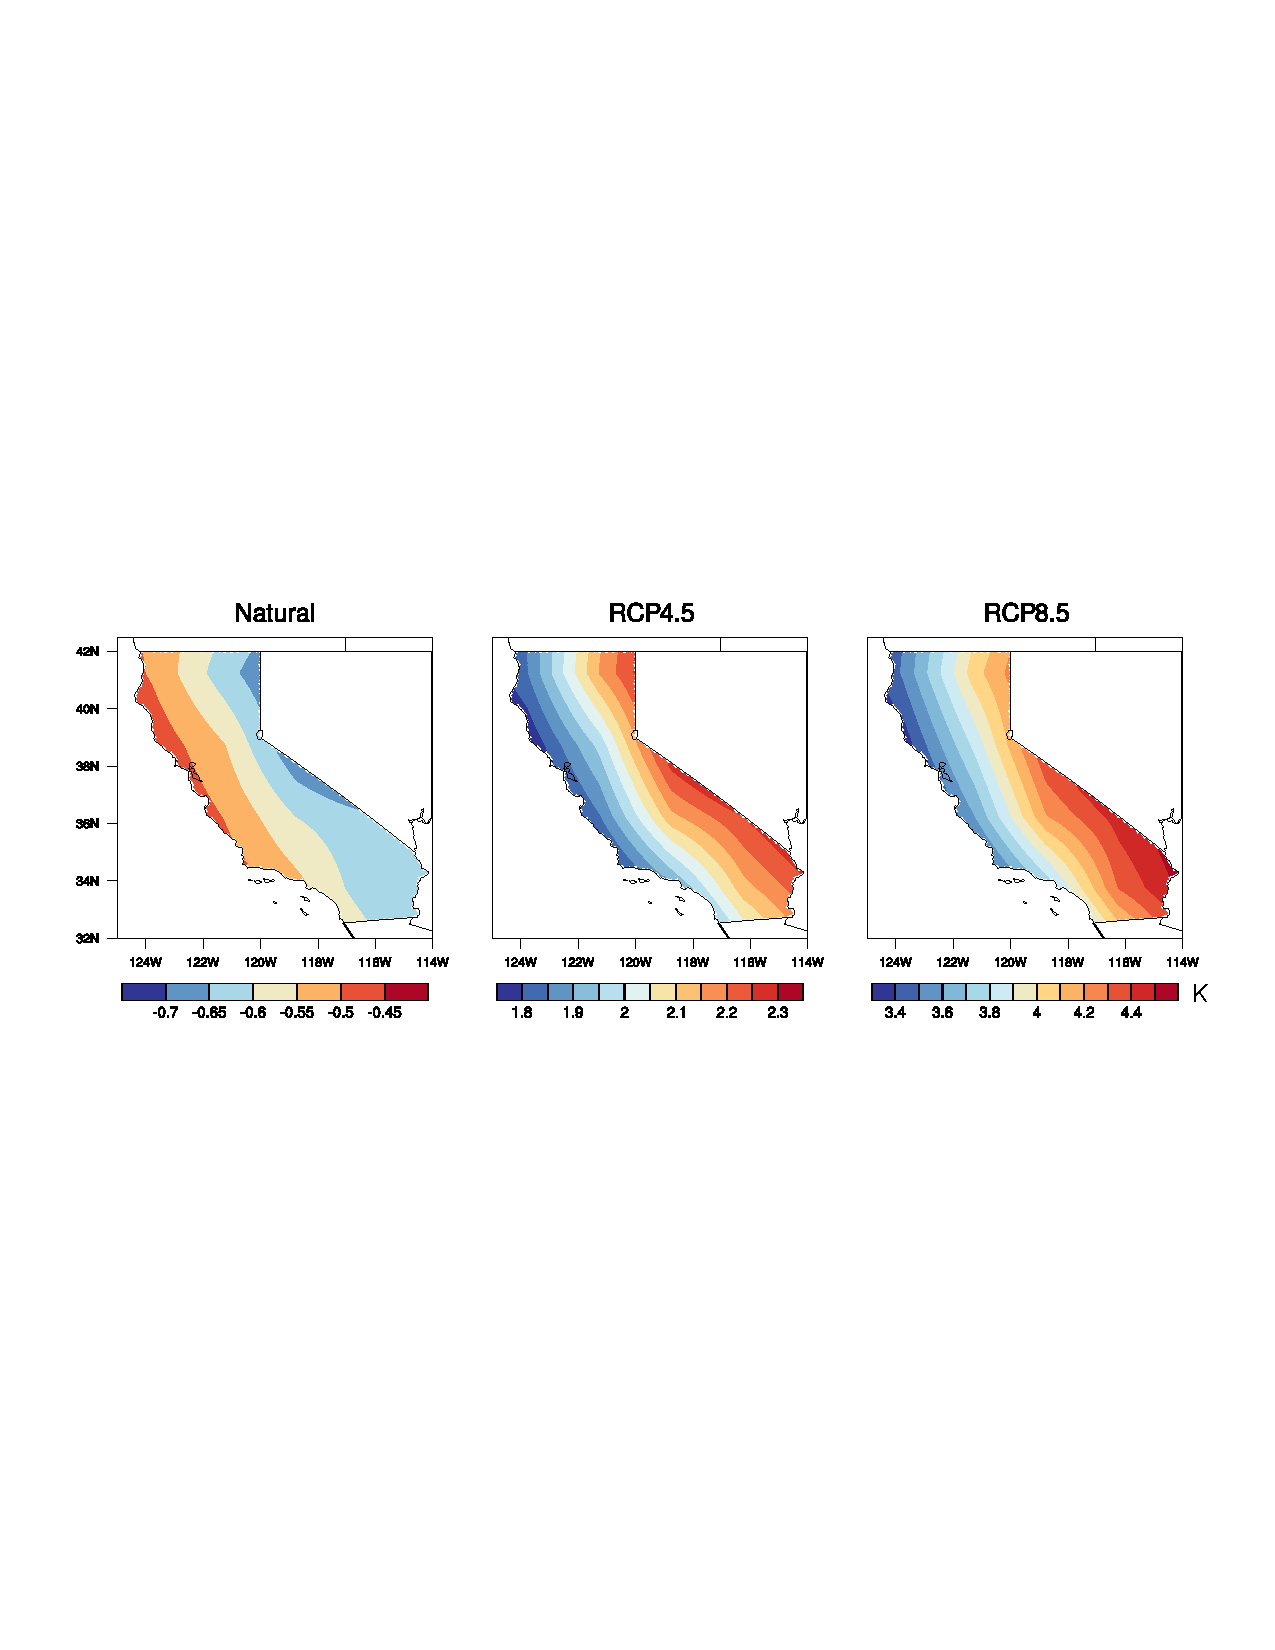
\includegraphics[width=6in]{FigS1.pdf}
\caption{Warming patterns averaged from Oct. to March. based on the CMIP5 ensemble mean compared to the recent historical for the natural, RCP4.5, and RCP8.5.}
\end{center}
\end{figure}

%precipitation and April 1st SWE from WRF at 27 km, and the 

\begin{figure}
\setfigurenum{S2}
\begin{center}
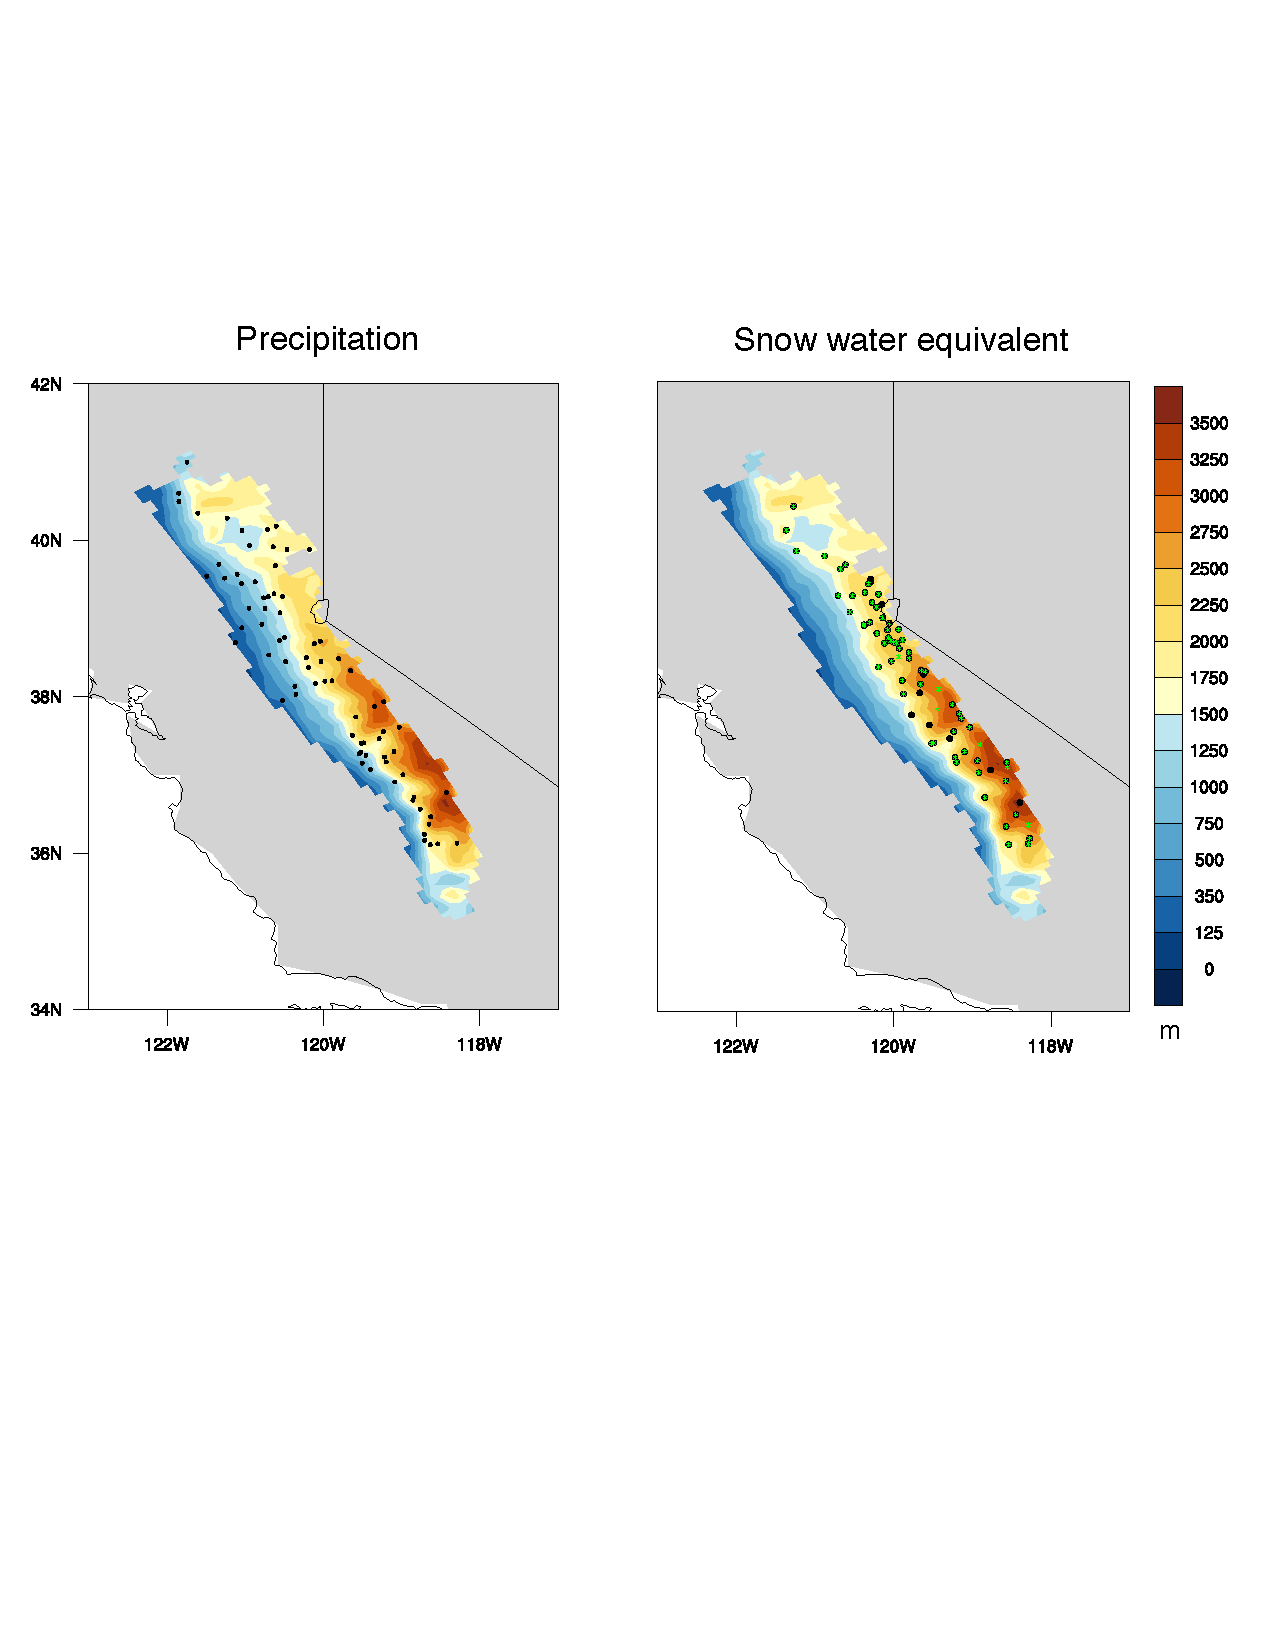
\includegraphics[width=6in]{FigS2.pdf}
\caption{Station locations for the observed precipitation and April 1st SWE (note: for the SWE, the black dots refer to the stations with data of the season 2015-2016 and green stars refer to the ones of the season 2016-2017).}
\end{center}
\end{figure}


\begin{figure}
\begin{center}
\setfigurenum{S3}
\includegraphics[width=6in, trim={0.2cm 4.0cm 0.2cm 3.0cm},clip]{FigS3.pdf}
\caption{Upper panel: (a) Scatter plot of October 1 to April 1 averaged precipitation according to the station observations and the corresponding simulated values over the Sierra Nevada (blue dots correspond to the water year 2015$-$2016 and red dots correspond to the water year 2016$-$2017; The black dashed line y = x is also depicted.); (b) Similar as (a), but for the April 1st SWE. Lower panel: (c) The spatial pattern of the average precipitation over Oct. 1st to April 1st from the WRF reference run at 9 km masked over the Sierra Nevada; (d) Similar as (c), but for the April 1st SWE masked over the Sierra Nevada area above the foothill.}
\end{center}
\end{figure}


\begin{figure}
\setfigurenum{S4}
\begin{center}
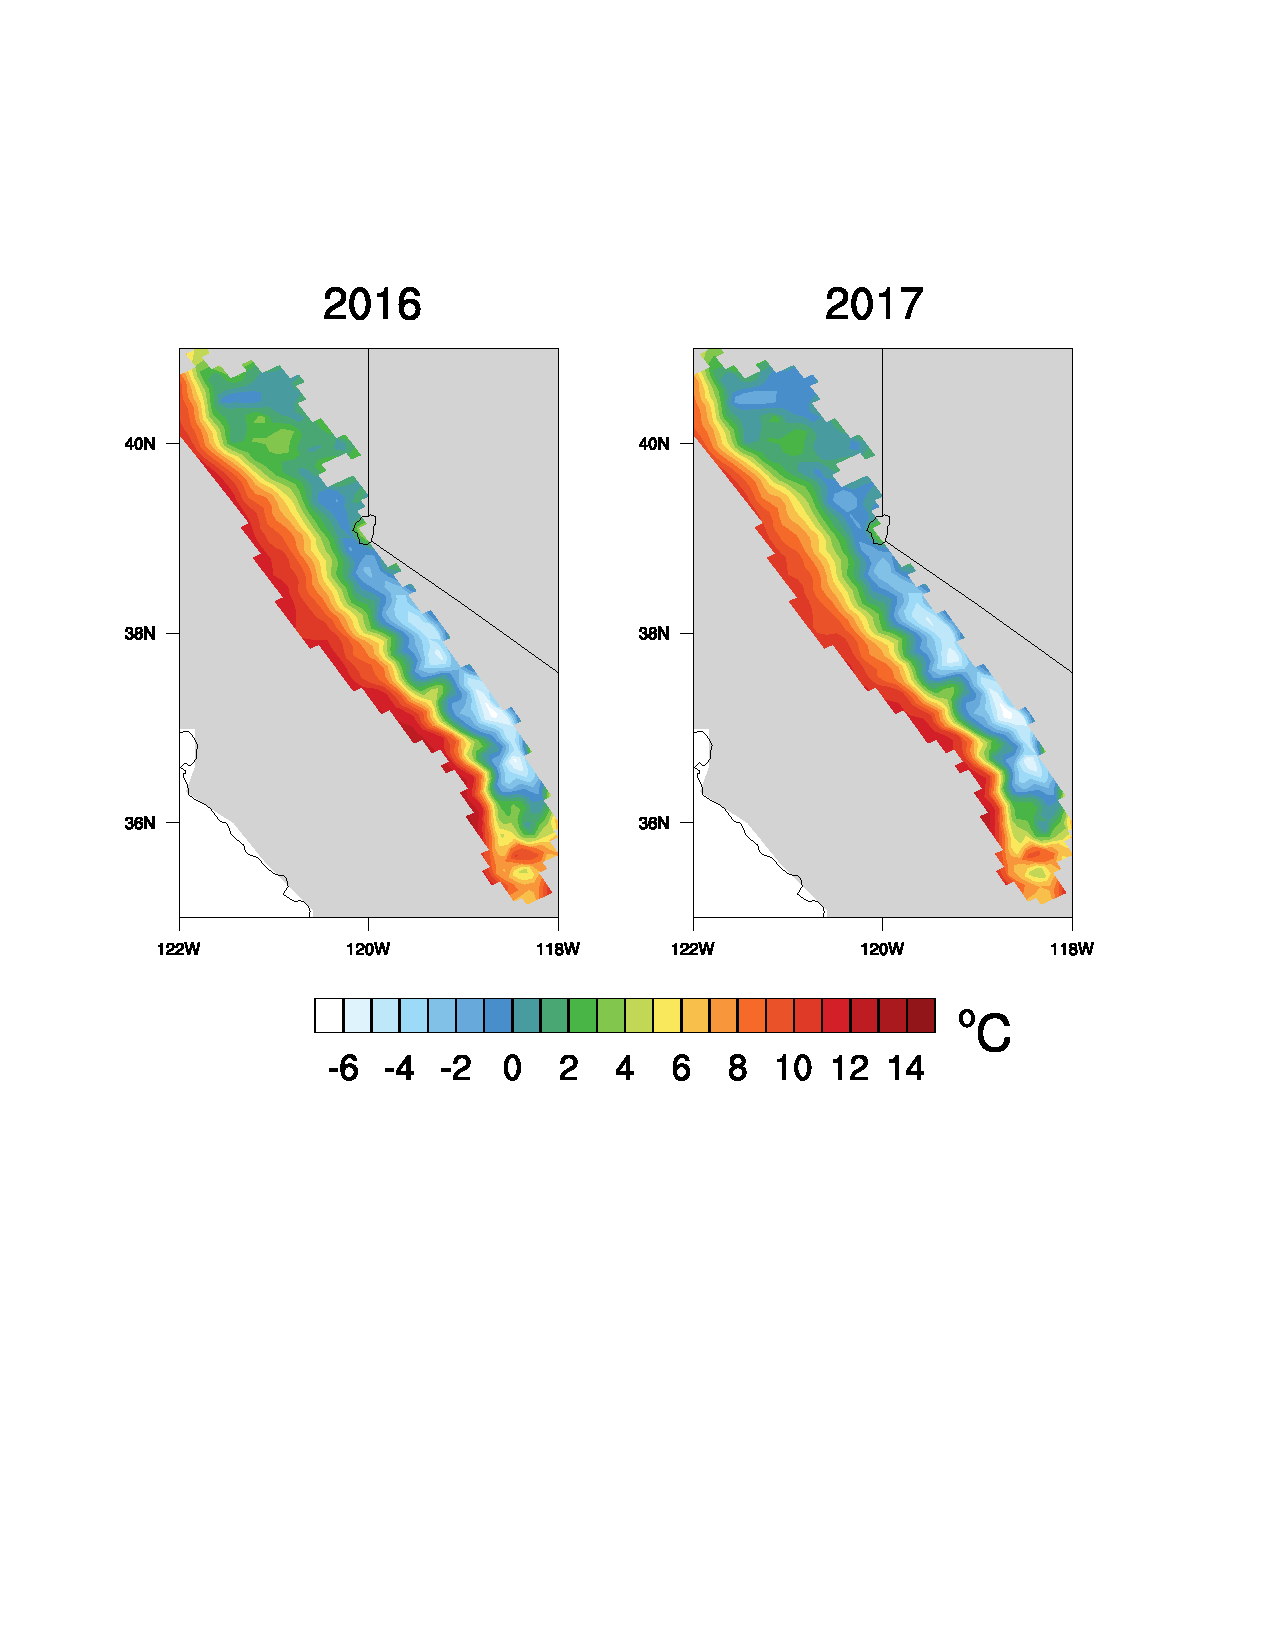
\includegraphics[width=6in]{FigS4.pdf}
\caption{Averaged near-surface temperature from WRF at 9km for the seasons 2015-2016 and 2016-2017 over Oct. to March.}
\end{center}
\end{figure}


\end{document}

